\section{Topic Tree}
\subsection{Overview}
Most learning management systems do not have a simple and easy method to import course material and resources from other courses. Some LMS platforms such as OpenLearning have no method of importing any data at all, and other platforms such as Canvas allows you to import crowd sourced material into your own course, however still does not allow you to import topics of resources. \\

This new LMS will have a new topic tree feature, which will allow teachers and academics to add course material under a specific topic instead.\\
Each topic will have prequisites of other topics, for example the topic Graphs will be a prequisite for the topic Depth first Search.\\

\begin{figure}[h!]
    \centering
    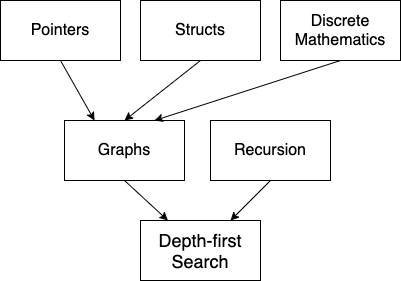
\includegraphics[scale=0.4]{topic-tree-example}
    \caption{Example of a topic tree with Depth first search}
\end{figure}

